% ---------------------------------------------------------------------------------------------------
% Experiments section.  \input this file into the main paper.
%   Packages: graphicx, booktabs, amsmath, amssymb, natbib (or adapt \citep).
%   Figures : fig_real/fig_toy_logscore.pdf, fig_real/fig_toy_stats.pdf, fig_real/fig_eeg.png and fig_real/fig_finance.png (7.4in wide rasters)
%             (regenerate with experiments/paper_figs.py)
%   Labels expected from the appendix: app:toys, app:eeg, app:finance, app:selection.
%   Citation keys used (rename to your .bib): chen2010shrinkage, ledoit2020analytical, gavish2014optimal,
%             goldberger2000physionet, schalk2004bci2000, barachant2012multiclass.
% ---------------------------------------------------------------------------------------------------
\providecommand{\scsi}{\textsc{SC-SI}}
\providecommand{\Ce}{C_{\mathrm{e}}}

\section{Experiments}
\label{sec:experiments}

We ask three questions, ordered by how much ground truth is available.
\textbf{(i)}~When the posterior is known exactly, does self-consistent training from noisy covariances alone recover it (\S\ref{sec:exp-toys})?
\textbf{(ii)}~On real covariance data with no ground truth, are the learned posteriors calibrated on held-out subjects (\S\ref{sec:exp-eeg})?
\textbf{(iii)}~Does the posterior improve a downstream decision, and does it stay calibrated as market regimes change (\S\ref{sec:exp-fin})?
In every experiment the learner sees only noisy empirical covariances $\Ce$ produced by the known Wishart channel; clean covariances are never used, not even for model selection.

\paragraph{Baselines and protocol shared by all experiments.}
We compare against the sample covariance, OAS linear shrinkage~\citep{chen2010shrinkage}, Ledoit--Wolf analytical nonlinear shrinkage (LW-NLS)~\citep{ledoit2020analytical}, and a conjugate inverse-Wishart prior fitted by marginal likelihood (IW-ML), the standard parametric Bayesian baseline.
A point estimator becomes a predictive law by adding Wishart channel noise around the estimate; it carries no estimation uncertainty of its own.
On a finite ensemble, self-consistent EM eventually over-sharpens the learned prior, so the outer iteration $k$ must be selected.
We select it on held-out validation pairs $(\Ce^{\mathrm{cal}},\Ce^{\mathrm{val}})$ that share a latent covariance, with a \emph{worst-case PIT score}: for a small set of functionals of $C$ (log-determinant, log condition number, top-eigenvalue share, an off-diagonal correlation, and the variance along the top and bottom empirical eigenvectors), we push posterior draws given $\Ce^{\mathrm{cal}}$ through the channel, compute the probability integral transform (PIT) of the observed $\Ce^{\mathrm{val}}$ functional, and keep the iteration with the smallest worst-case Kolmogorov--Smirnov distance to uniformity.
Unlike the aggregate predictive log-score, this score cannot trade one functional against another (Appendix~\ref{app:selection}).
It needs no ground truth, so it applies unchanged to real data.

% =====================================================================================================
\subsection{Toy models with oracles}
\label{sec:exp-toys}

\paragraph{Setting and aim.}
We use four $d{=}8$ priors whose posterior $P(C\mid \Ce)$ is available as an oracle.
Two are inverse-Wishart, rotationally invariant (RI, $N{=}40$) or with an anisotropic scale matrix of condition number 16 (non-RI, $N{=}28$); conjugacy makes their posterior exact.
The third is a two-factor model $C=BB^\top+\mathrm{diag}(\psi)$ ($N{=}28$) with a non-conjugate posterior, computed by Hamiltonian Monte Carlo ($\hat R\le 1.02$).
The fourth is not rotationally invariant and lives on a one-parameter curve of covariances: the AR(1) family $C_{ij}=e^{-\gamma|t_i-t_j|}$, $t_i=i/4$, $\log\gamma\sim\mathcal N(0,0.5^2)$ ($N{=}40$).
The learner is never told the family, and its posterior is a one-dimensional integral over $\gamma$, computed exactly by quadrature (validated by simulation-based calibration).
\scsi{} sees only noisy covariances: $M{=}2000$--$3000$ per prior, and $M{=}8000$ for AR(1), whose thin posterior needs $K{=}120$ EM iterations rather than 24.
The aim is to measure how close a learner that never observes a clean $C$ gets to the oracle, and whether it beats the parametric IW-ML baseline exactly when that baseline is misspecified.
We report (a)~the held-out predictive log-score of $\Ce^{\mathrm{val}}$ given $\Ce^{\mathrm{cal}}$, relative to the oracle, and (b)~the Wasserstein-1 distance between the learned and oracle posteriors of six statistics of $C$, in units of the oracle's posterior standard deviation, averaged over 128 held-out tasks (sampling floor $0.055$; details in Appendix~\ref{app:toys}).

\begin{figure}[t]
  \centering
  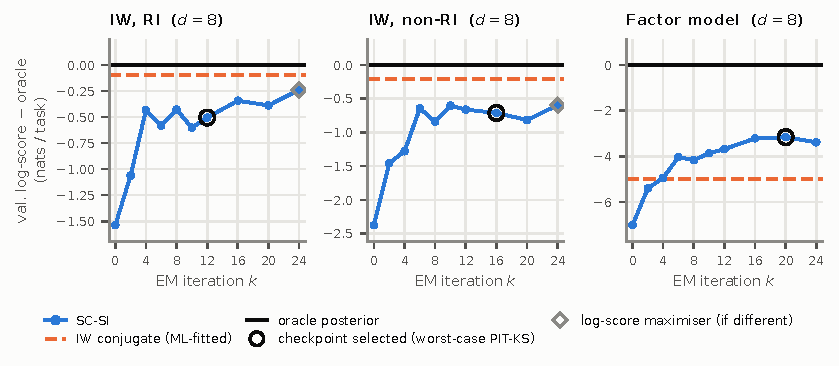
\includegraphics[width=\linewidth]{fig_real/fig_toy_logscore.pdf}
  \caption{\textbf{Self-consistent training approaches the oracle.}
  Held-out predictive log-score relative to the oracle posterior (300 validation pairs, nats per task) along EM iterations $k$; $k{=}0$ is the deconvolved log-Gaussian initialisation.
  Dashed: IW-ML.
  Circle: checkpoint selected by the worst-case PIT score; diamond: log-score maximiser, when different.
  AR(1) is trained for $K{=}120$ iterations, the other priors for 24.
  The sample-covariance plug-in lies 14--26 nats below the oracle (off scale).}
  \label{fig:toy-logscore}
\end{figure}

\paragraph{Results.}
\textbf{EM closes most of the gap to the oracle.}
From the initialisation at $k{=}0$, self-consistent iterations close 67\%, 70\%, 55\% and 96\% of the log-score gap to the oracle on the RI, non-RI, factor and AR(1) priors (Fig.~\ref{fig:toy-logscore}).
\textbf{Where the parametric family is right it wins; where it is wrong, \scsi{} does.}
On the conjugate priors IW-ML is exact by construction (0.1--0.2 nats from the oracle), and \scsi{} trails it by 0.4--0.5 nats: the price of not knowing the family.
On the factor model the ordering flips: IW-ML sits 5.0 nats below the oracle and \scsi{} 3.2, a gain of 1.8 nats.
On the AR(1) family, which no inverse-Wishart can follow, the gap is far larger: IW-ML is 8.5 nats below the oracle, \scsi{} 0.5, a gain of 8 nats per task.

\begin{figure}[t]
  \centering
  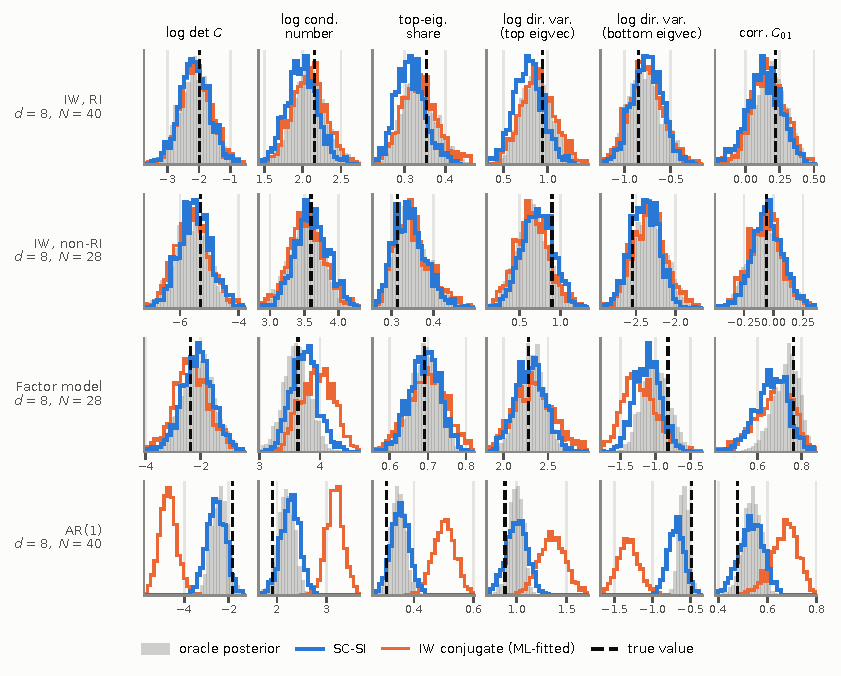
\includegraphics[width=\linewidth]{fig_real/fig_toy_stats.pdf}
  \caption{\textbf{Posterior of six statistics of $C$ on the four toy priors.}
  Draws for the test task with median error (median over 128 tasks of the mean $W_1$ across statistics), not selected for appearance; dashed line: true value.
  Aggregate distances over all 128 tasks are in Table~\ref{tab:toy-w1}.}
  \label{fig:toy-stats}
\end{figure}

\begin{table}[t]
  \centering
  \caption{\textbf{Log-score and distance to the oracle posterior.}
  Log-score: held-out predictive log-score of $\Ce^{\mathrm{val}}$ given $\Ce^{\mathrm{cal}}$ in nats per task (300 validation pairs, 64 posterior draws, as in Fig.~\ref{fig:toy-logscore}; \scsi{} at its selected checkpoint).
  $W_1$: Wasserstein-1 distance to the oracle posterior in units of its s.d., mean over 128 held-out tasks (sampling floor $0.055$).
  $\kappa$: condition number; $\mathrm{dv}$: log variance along the top/bottom empirical eigenvector of $\Ce$; $C_{01}$: correlation of the first two coordinates.
  Arrows give the better direction; bold: best of the two methods in each block (the oracle is the reference).}
  \label{tab:toy-w1}
  \footnotesize
  \setlength{\tabcolsep}{2.8pt}
  \begin{tabular}{@{}llcccccccc@{}}
    \toprule
     & & & \multicolumn{7}{c}{$W_1$ to the oracle posterior $\downarrow$} \\
    \cmidrule(l){4-10}
    Prior & Method & log-score $\uparrow$ & $\log\det C$ & $\log\kappa$ & top share & $\mathrm{dv}_{\mathrm{top}}$ & $\mathrm{dv}_{\mathrm{bot}}$ & $C_{01}$ & mean \\
    \midrule
    IW, RI & \scsi{} & $-134.27$ & 0.26 & 0.42 & 0.43 & 0.47 & 0.35 & 0.23 & 0.36 \\
     & IW-ML & $\mathbf{-133.86}$ & \textbf{0.05} & \textbf{0.05} & \textbf{0.05} & \textbf{0.05} & \textbf{0.05} & \textbf{0.05} & \textbf{0.05} \\
     & Oracle & $-133.76$ & -- & -- & -- & -- & -- & -- & -- \\
    \midrule
    IW, non-RI & \scsi{} & $-53.46$ & 0.23 & 0.22 & 0.23 & 0.25 & 0.31 & 0.22 & 0.24 \\
     & IW-ML & $\mathbf{-52.95}$ & \textbf{0.05} & \textbf{0.05} & \textbf{0.05} & \textbf{0.05} & \textbf{0.05} & \textbf{0.05} & \textbf{0.05} \\
     & Oracle & $-52.75$ & -- & -- & -- & -- & -- & -- & -- \\
    \midrule
    Factor model & \scsi{} & $\mathbf{-93.05}$ & \textbf{0.27} & \textbf{0.70} & \textbf{0.32} & \textbf{0.29} & \textbf{0.90} & \textbf{0.35} & \textbf{0.47} \\
     & IW-ML & $-94.89$ & \textbf{0.27} & 1.00 & 0.65 & 0.85 & 1.15 & 0.45 & 0.73 \\
     & Oracle & $-89.89$ & -- & -- & -- & -- & -- & -- & -- \\
    \midrule
    AR(1) & \scsi{} & $\mathbf{-27.63}$ & \textbf{0.22} & \textbf{0.56} & \textbf{0.33} & \textbf{1.23} & \textbf{0.83} & \textbf{0.54} & \textbf{0.62} \\
     & IW-ML & $-35.68$ & 2.57 & 2.78 & 2.65 & 4.01 & 3.57 & 3.01 & 3.10 \\
     & Oracle & $-27.15$ & -- & -- & -- & -- & -- & -- & -- \\
    \bottomrule
  \end{tabular}
\end{table}

\textbf{The posterior is accurate on the statistics that matter.}
On the IW priors \scsi{} lies within 0.2--0.5 oracle standard deviations on all six statistics (Fig.~\ref{fig:toy-stats}, Table~\ref{tab:toy-w1}); the hardest are the spectrum-shape statistics of the RI prior, where its posterior is slightly too narrow (s.d.\ ratio $0.85$--$0.94$).
On the factor model \scsi{} is closer to the oracle than IW-ML on five of six statistics and tied on $\log\det C$ (mean $0.47$ vs.\ $0.73$), by $1.4$--$2.9\times$ on the log condition number, the top-eigenvalue share and the top-direction variance, the statistics that depend on the shape of the spectrum, where a misspecified conjugate family has little freedom.
The largest residual errors remain the log condition number and the bottom-direction variance ($0.70$, $0.90$), where IW-ML is worse still.

\textbf{On a non-invariant prior the margin is largest, and it is set by the number of EM iterations, not by the data.}
On AR(1), IW-ML is $2.6$--$4.0$ oracle standard deviations from the oracle on every statistic (mean $3.10$); \scsi{} is $0.22$--$1.23$ (mean $0.62$), $3.3$--$12\times$ closer, with a posterior slightly too wide (mean s.d.\ ratio $1.45$, and $2.3$ for the top-direction variance, the largest residual).
The residual is not a capacity limit: the same network trained on clean $(C,\Ce)$ pairs (supervised control, 52k steps) reaches a mean $W_1$ of $0.17$.
It is the length of the self-consistent loop: at $M{=}8000$ the mean $W_1$ falls from $1.10$ ($K{=}24$) to $0.76$ ($K{=}60$) and $0.62$ ($K{=}120$), still decreasing.
The training-set size hardly matters: at $K{=}60$, $M{=}2000$, $8000$ and $32000$ give $0.80$, $0.76$ and $0.75$, so even $M{=}2000$ is $3.9\times$ closer than IW-ML ($3.11$), and doubling the number of SDE steps changes nothing ($0.76$).

\textbf{Selection matters.}
The aggregate log-score and the worst-case PIT score pick different checkpoints (Fig.~\ref{fig:toy-logscore}, circle vs.\ diamond).
On the RI prior the log-score maximiser ($k{=}24$) is worse than our pick ($k{=}12$) on all six statistics (mean $W_1$ $0.50$ vs.\ $0.36$; log condition number $0.72$ vs.\ $0.42$), and likewise on the non-RI prior ($0.28$ vs.\ $0.24$).
On AR(1) both criteria select the last iteration, so no over-sharpening has set in within $K{=}120$.
The gap widens with dimension: at $d{=}20$ the log-score maximiser has a log-condition-number distance of $1.51$ against $0.33$ for our pick (Appendix~\ref{app:toys}).
Accuracy also degrades with dimension: at $d{=}20$ the top-eigenvalue share and the top- and bottom-direction variances remain $1.1$--$1.4$ oracle standard deviations off even at the selected checkpoint, so we regard scaling the general algorithm beyond $d\approx 10$ as open.

% =====================================================================================================
\subsection{EEG: calibrated uncertainty for held-out subjects}
\label{sec:exp-eeg}

\paragraph{Setting and aim.}
We use the PhysioNet EEG Motor Movement/Imagery dataset~\citep{goldberger2000physionet,schalk2004bci2000}: 109 subjects, resting eyes-open and eyes-closed runs, 8 channels (Fz, C3, Cz, C4, Pz, O1, Oz, O2), alpha band (8--13\,Hz), split into non-overlapping 4-s windows ($d{=}8$).
Band-limited samples are serially correlated, so we use an effective $N{=}28$ ($N/d{=}3.5$), set from test--retest variability of half-windows on training subjects (Appendix~\ref{app:eeg}).
The prior is learned from the 1960 unlabeled window covariances of 70 training subjects (both conditions pooled); 10 validation subjects select the checkpoint and 29 held-out subjects are used for testing.
The aim is to test whether the learned posterior is a calibrated predictive law on \emph{unseen subjects}, and whether this helps a decision.

\paragraph{Protocols and metrics.}
For each test window we compute the posterior from a calibration window and score the predictive law of a validation window, under two protocols: \emph{split-half}, where both windows are interleaved 1-s chunks of the same 8-s epoch and thus share one covariance (isolating estimation uncertainty; 812 cases), and \emph{next window}, where the covariance may drift (754 cases).
We report the predictive log-score, the coverage of central predictive intervals for directional variances and for nonlinear functionals of $C$, and eyes-open vs.\ eyes-closed classification from a single window with a logistic regression on tangent-space features~\citep{barachant2012multiclass}, using either the plug-in covariance or the average prediction over posterior draws.
Classification is cross-validated over all 109 subjects (5 subject-disjoint folds, each with its own prior, classifier and checkpoint) so that every subject is tested once; the other analyses use the 29 held-out subjects.

\begin{figure}[t]
  \centering
  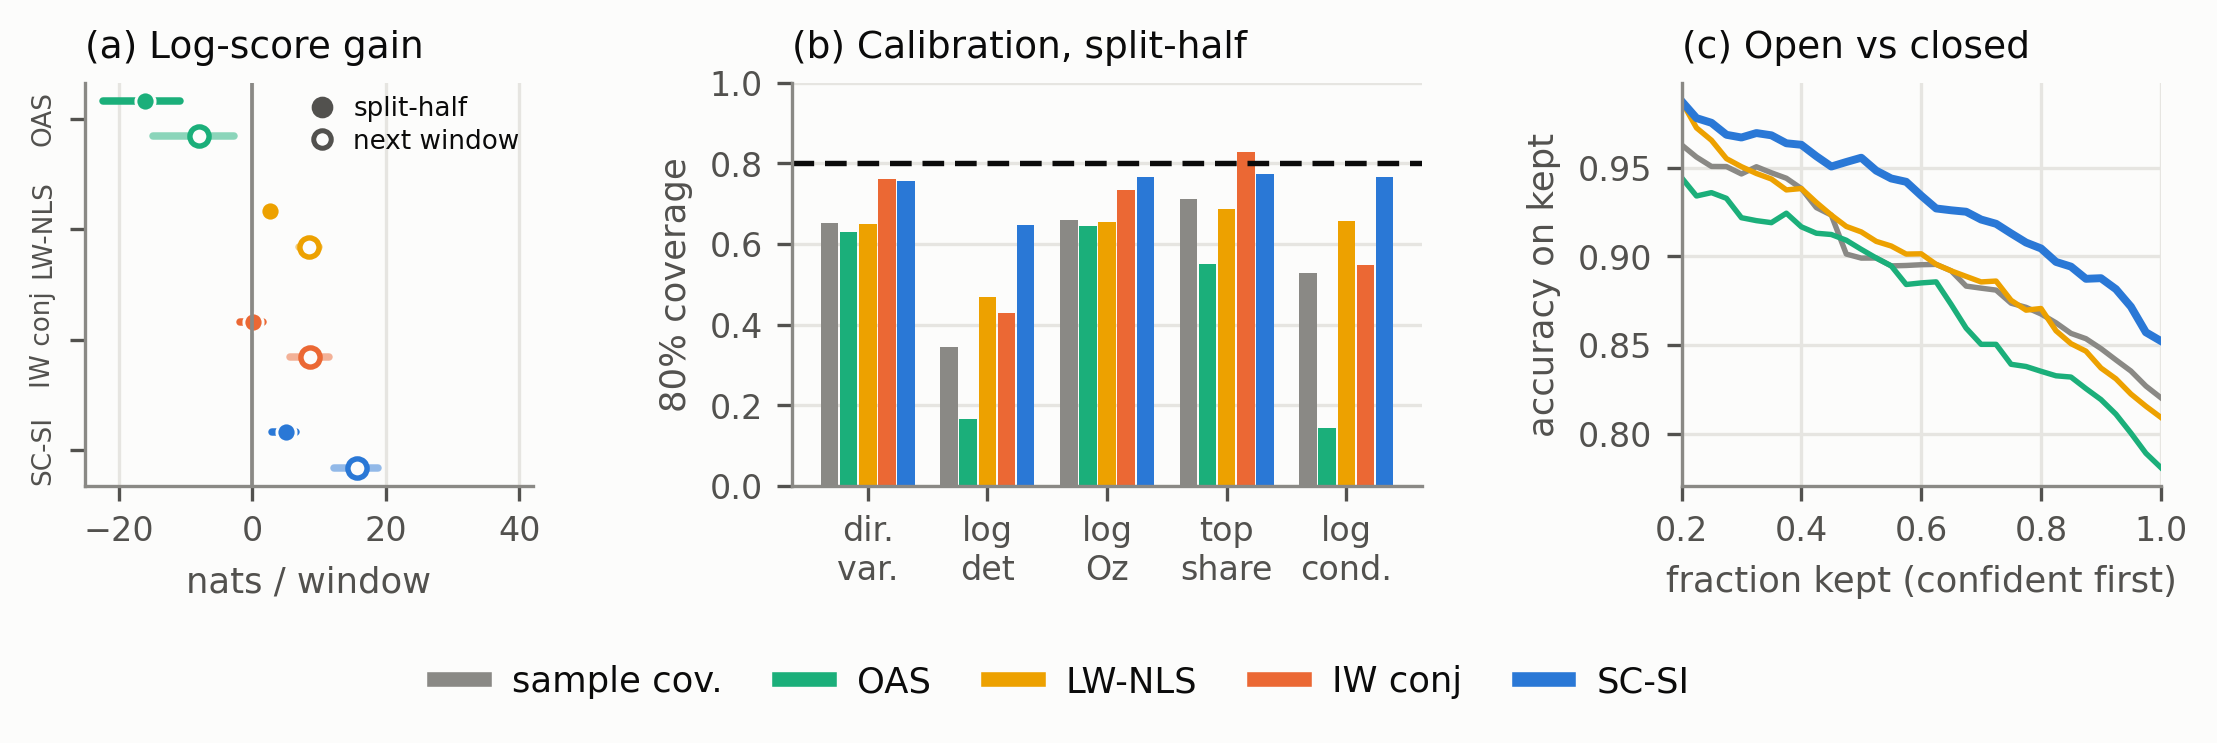
\includegraphics[width=\linewidth]{fig_real/fig_eeg.png}
  \caption{\textbf{EEG on held-out subjects.}
  Panels (a) and (b) use the 29 held-out test subjects.
  (a)~Predictive log-score gain over the sample covariance with 95\% subject-level bootstrap intervals; filled: split-half, hollow: next window.
  (b)~Coverage of the central 80\% predictive interval (dashed: nominal) for directional variances (channel axes and top pooled PCs) and four functionals of $C$ (log det: log-determinant; log Oz: log power at Oz; top share: top-eigenvalue share; log cond.: log condition number), split-half; dir.\ var.: directional variances.
  (c)~Accuracy of eyes-open vs.\ eyes-closed classification when only the most confident windows are kept, from 5-fold subject-disjoint cross-validation over all 109 subjects; SC-SI uses the posterior-averaged classifier, the others plug-in features.}
  \label{fig:eeg}
\end{figure}

\paragraph{Results.}
\textbf{Log-score.}
In the split-half test \scsi{} gains $+5.0$ nats per window over the sample covariance (95\% CI $[3.0,6.5]$), against $+2.8$ for LW-NLS, $+0.1$ for IW-ML and $-16.0$ for OAS (Fig.~\ref{fig:eeg}a).
The paired margin over the strongest point estimator, LW-NLS, is $+2.3$ $[0.4,3.6]$ nats.
The ranking is preserved when the covariance drifts between windows ($+15.7$ for \scsi{} vs.\ $+8.6$ LW-NLS, $+8.7$ IW-ML, $-7.9$ OAS).
\textbf{Calibration.}
For directional variances the 80\% intervals of \scsi{} and IW-ML are close to nominal ($0.76$ each, at 50/80/95\%: $0.47/0.76/0.91$ and $0.46/0.76/0.92$), whereas the plug-ins under-cover ($0.63$--$0.65$ at 80\%).
The two Bayesian methods separate on spectrum-dependent functionals (Fig.~\ref{fig:eeg}b): the 80\% interval of the log-determinant covers $0.65$ for \scsi{} against $0.43$ for IW-ML and $0.17$--$0.47$ for the plug-ins; for the log condition number, $0.77$ against $0.55$ and $0.14$--$0.66$.
This is consistent with a conjugate prior's single concentration parameter being too rigid for the spectrum.
IW-ML is better on the top-eigenvalue share ($0.83$ vs.\ $0.77$), and every method under-covers the open-vs-closed Riemannian distance ($0.26$--$0.41$, \scsi{} highest; not shown, Appendix~\ref{app:eeg}).
\textbf{Decisions.}
Averaging predictions over posterior draws gives a small gain in eyes-open vs.\ eyes-closed classification when every subject is tested once (Fig.~\ref{fig:eeg}c).
Accuracy is $0.806$ against $0.781$--$0.792$ for the plug-ins, and the negative log-likelihood $0.443$ against $0.464$--$0.492$.
Paired subject-level bootstrap intervals put the accuracy gain at $+1.4$ $[0.1,2.8]$ points over the sample covariance, $+1.5$ $[0.0,3.0]$ over LW-NLS and $+2.6$ $[0.4,4.6]$ over OAS, with \scsi{} ahead in 3, 4 and 5 of the 5 folds.
Keeping the 50\% most confident windows helps against OAS ($+3.7$ points) but not against the sample covariance or LW-NLS (intervals include zero).
The larger gains seen on a single 29-subject split ($+3$ to $+4$ points) do not carry over to the whole cohort, so we regard the classification benefit as small.

\paragraph{Takeaway.}
On unseen subjects the learned posterior is a calibrated predictive law for first-order quantities and, unlike a fitted conjugate prior, for spectrum-dependent functionals; the downstream classification benefit is small.

% =====================================================================================================
\subsection{Financial returns: decisions across market regimes}
\label{sec:exp-fin}

\paragraph{Setting.}
We use daily value-weighted returns of the 48 Ken French industry portfolios (1926--2026), with a zero-mean model.
A task is a 63-day window and a random basket of $d{=}12$ industries observed throughout the window.
The prior is learned from past windows only (non-overlapping windows, 16 random baskets each, $M\approx 4.5$--$5.7$k) and refit on three expanding folds; test months are 1995--2004, 2005--2014 and 2015--2026, with 8 fixed baskets and monthly forecasts (3008 cases).
The effective sample size is calibrated on a validation fold that precedes all test folds, by maximising the calibration of forward intervals for IW-ML: $N{=}19$ for the 63-day window and $6$ for the 21-day forward window ($N/d{=}1.6$).
It is not a sampling count; it inflates forecast uncertainty and absorbs drift between estimation and forecast windows (Appendix~\ref{app:finance}).

\paragraph{Aim and estimators.}
The aim is to test the posterior on a decision and on its calibration through time.
The decision is the global minimum-variance portfolio built from each estimator, scored by its realised variance over the next 21 days relative to OAS.
Estimators are the covariance estimates of \S\ref{sec:experiments}, the \scsi{} and IW-ML posterior means, the \scsi{} Stein-optimal covariance (inverse of the posterior mean of the inverse), and PCA factor models whose number of factors $K$ is chosen by the Gavish--Donoho threshold~\citep{gavish2014optimal} or by the Bayes rule minimising posterior expected Stein loss.

\paragraph{Checkpoint selection.}
Because the forward window has fewer effective observations than assets, a simulated forward covariance is rank-deficient and the log-determinant and condition number carry no information.
The worst-case PIT score therefore uses the top-eigenvalue share, a correlation and the top-direction variance.
It omits the bottom-direction variance, which a single window with $N/d{=}1.6$ is unlikely to identify.
We made this choice after inspecting validation curves; Appendix~\ref{app:selection} reports the all-functional variant.

\begin{figure}[t]
  \centering
  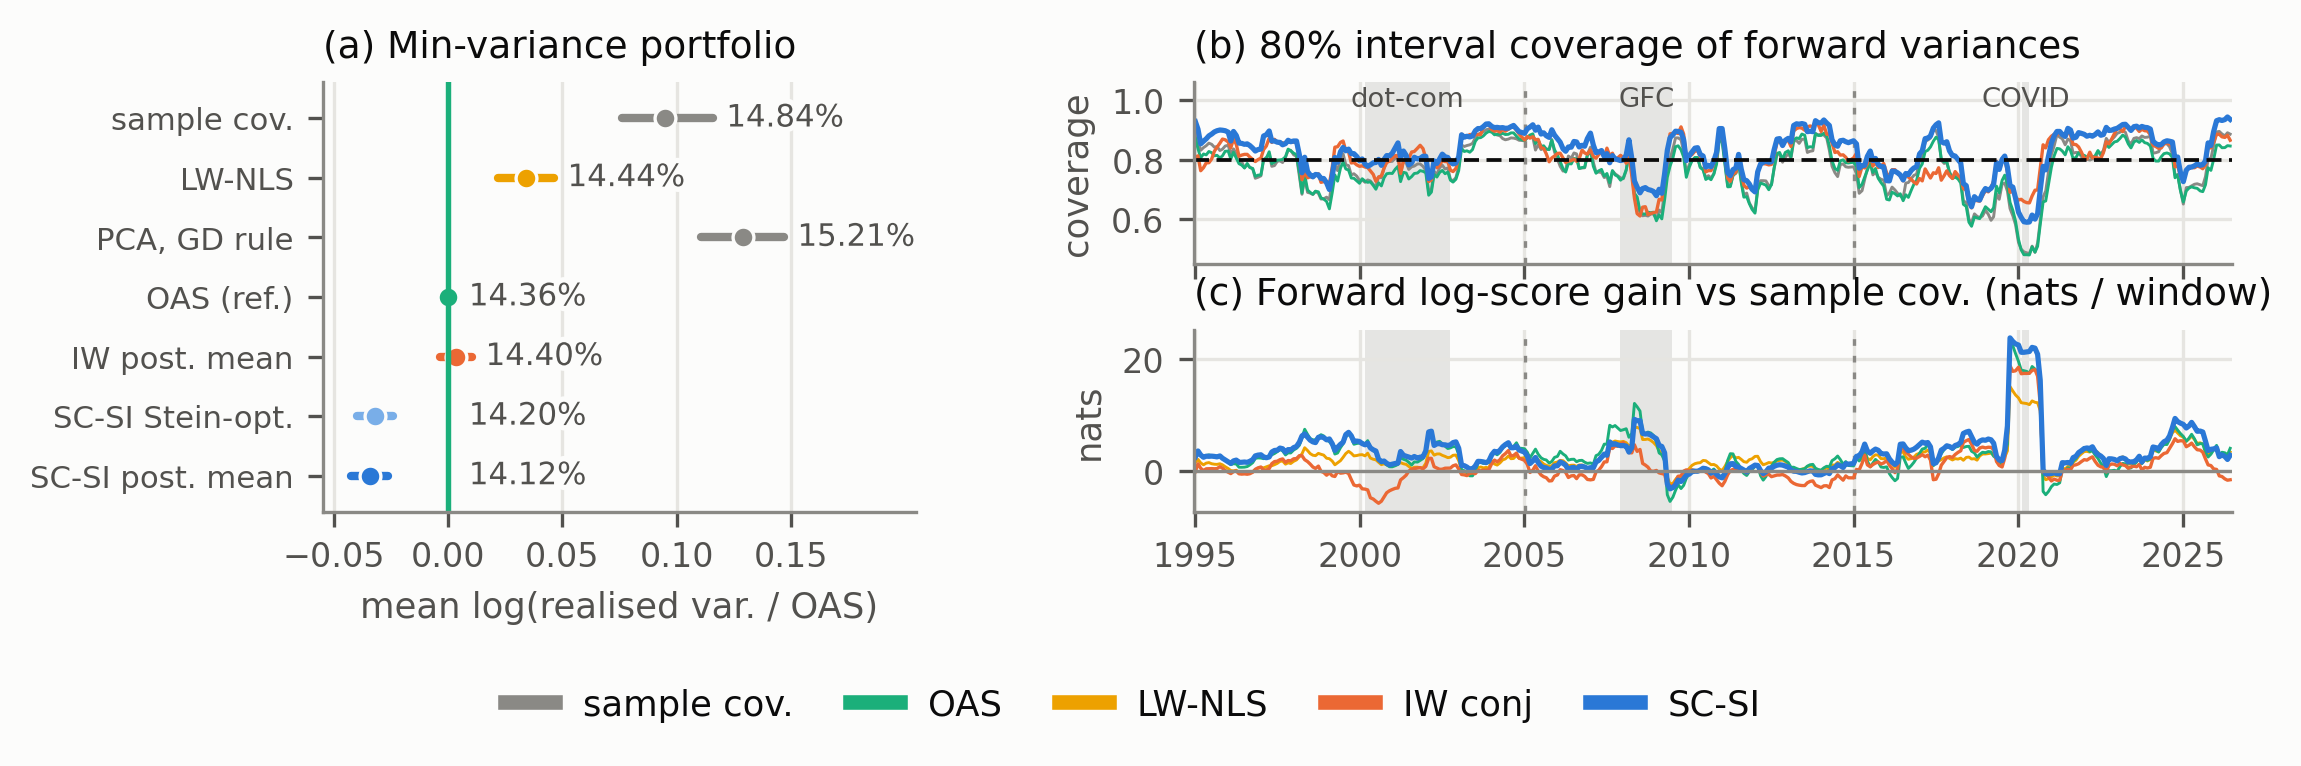
\includegraphics[width=\linewidth]{fig_real/fig_finance.png}
  \caption{\textbf{Financial returns, 1995--2026.}
  (a)~Out-of-sample minimum-variance portfolio: mean log ratio of realised 21-day variance to OAS with 95\% month-block bootstrap intervals (left is lower risk); post.\ mean: posterior-mean covariance, Stein-opt.: Stein-optimal covariance, PCA, GD rule: number of factors by the Gavish--Donoho threshold; the percentages give the annualised realised volatility of the portfolio.
  (b)~12-month rolling coverage of the central 80\% forward interval for the variances of the 12 assets and the equal-weight portfolio.
  (c)~12-month rolling forward predictive log-score gain over the sample covariance.
  Shaded: dot-com bust, global financial crisis and COVID; dotted: model refits (2005, 2015).
  All quantities are averaged over the 8 baskets of a month.}
  \label{fig:finance}
\end{figure}

\paragraph{Results.}
\textbf{The posterior improves the decision.}
Using the \scsi{} posterior mean as the covariance input lowers realised variance by $3.4\%$ relative to OAS (log ratio $-0.034$, 95\% CI $[-0.043,-0.026]$; annualised volatility $14.12\%$ vs.\ $14.36\%$), and the Stein-optimal covariance is close ($-0.032$; Fig.~\ref{fig:finance}a).
Every other estimator is at or above OAS: the IW-ML posterior mean ($+0.004$, not significant), LW-NLS ($+0.034$) and the sample covariance ($+0.095$).
The advantage is steady rather than driven by a few episodes: it holds in each volatility tercile ($-0.051$, $-0.022$, $-0.030$ from low to high; Appendix~\ref{app:finance}).
Using the posterior to pick the number of factors does not help: PCA with the \scsi{} Bayes rule is $+0.086$ above OAS (not shown), better than Gavish--Donoho ($+0.129$) or the IW-ML Bayes rule ($+0.119$) but far from the posterior mean.
The value lies in using the whole posterior, not in a hard rank decision.
\textbf{Calibration degrades in stress, less so for posterior-based laws.}
The 80\% coverage of forward variances falls for every method in the global financial crisis and in COVID (Fig.~\ref{fig:finance}b).
OAS and the sample covariance bottom out at $0.60$ and $0.48$--$0.49$, \scsi{} at $0.68$ and $0.59$, and IW-ML at $0.61$ and $0.66$.
By volatility tercile, \scsi{} covers $0.84/0.85/0.79$ (low/mid/high), IW-ML $0.81/0.81/0.79$, OAS $0.77/0.80/0.73$ and the sample covariance $0.77/0.81/0.75$: in the top tercile the plug-ins fall to $0.73$--$0.75$ while both posterior methods stay at $0.79$.
In calm markets \scsi{} is slightly conservative and IW-ML is closest to nominal.
\textbf{Log-score does not separate \scsi{} from OAS.}
Over the sample covariance, \scsi{} gains $+3.4$ nats $[2.3,4.8]$ per window against $+3.0$ $[1.8,4.7]$ for OAS, $+2.3$ for LW-NLS and $+1.0$ for IW-ML (Fig.~\ref{fig:finance}c).
Gains are concentrated in a few episodes, chiefly a spike shared by all methods in early 2020, and intervals overlap in every regime.
\textbf{Log-score and decision quality can disagree.}
Training to $K{=}30$ without stopping, which is close to what the aggregate log-score selects (iterations 30/25/30 in the three folds), raises the \scsi{} log-score gain to $+4.4$ $[3.3,5.8]$ but removes the portfolio advantage ($-0.003$, $[-0.015,+0.010]$).
A log-score stopping rule would therefore favour a model that is worse for the decision.
The all-functional selection rule of Appendix~\ref{app:selection} gives a posterior-mean log ratio of $-0.029$ and a log-score gain of $+0.1$.

\paragraph{Takeaway.}
The posterior is most useful used whole: as a covariance input it beats shrinkage for minimum-variance investing in every volatility regime, and its predictive intervals hold up better than plug-in intervals in stress, but the effect is modest ($\approx 3\%$ of variance), rests on an effective sample size tuned for forecasting, and depends on how the training iteration is selected.
